\section{The Minimal Axiom}
\label{sec:axiom}

VED is founded on a single, irreducible statement:

\begin{keybox}
\textit{There is difference.}
\end{keybox}

This is not a metaphor or a philosophical preamble.
It is a structural condition.
A perfectly symmetric system produces no gradients, no flows,
and no observable events.
Without asymmetry, nothing happens.
The overall structure is summarized in Fig.~\ref{fig:generative_chain}.

\begin{figure}[t]
\centering
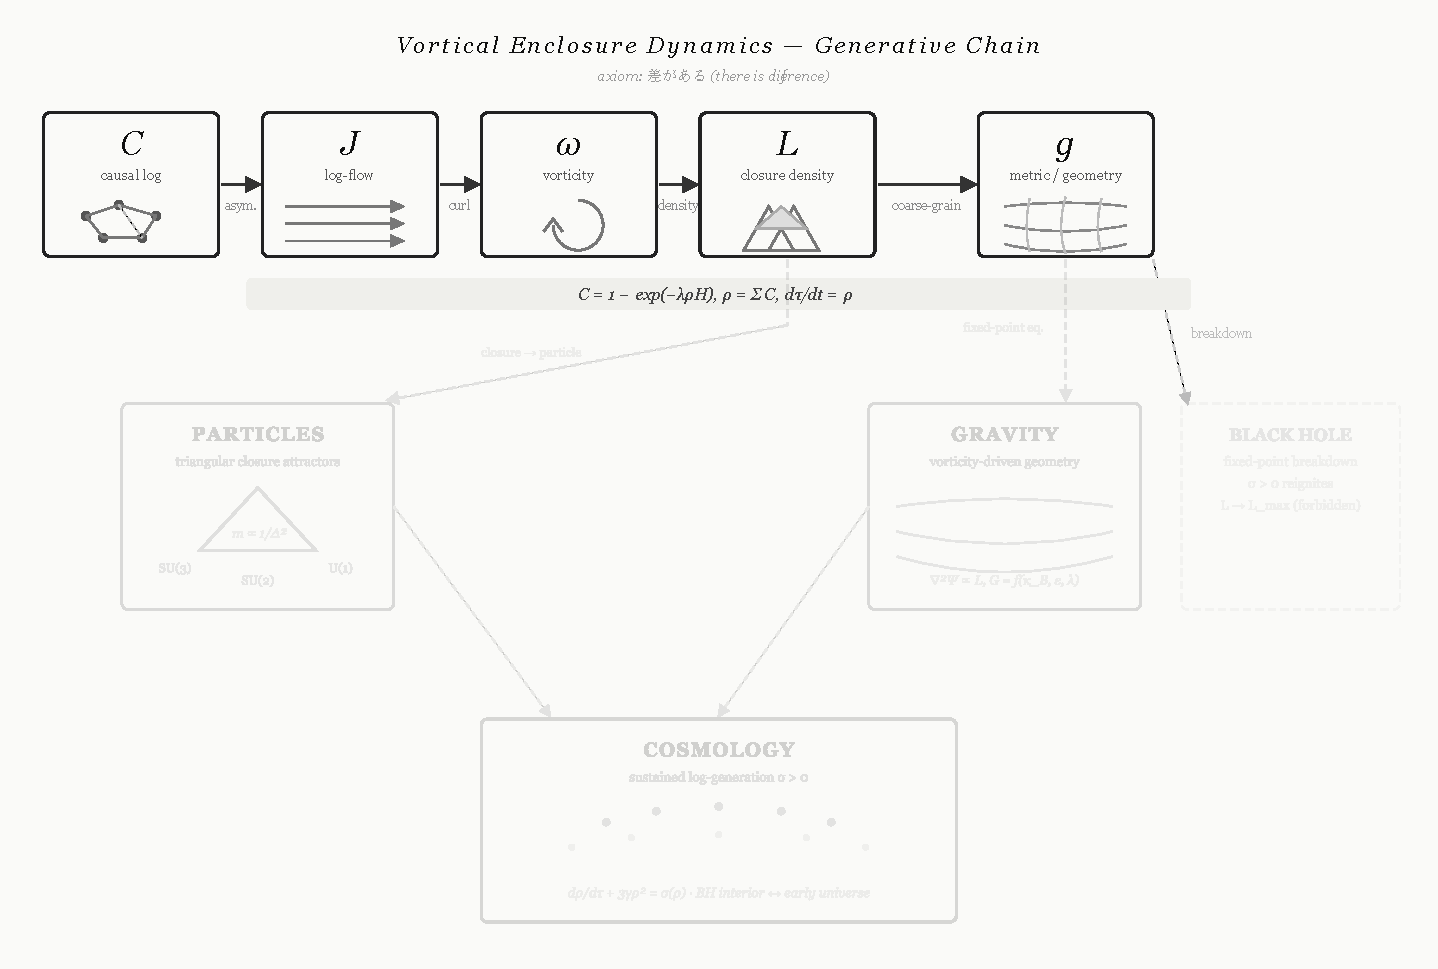
\includegraphics[width=0.9\linewidth]{figures/fig1_generative_chain.pdf}
\caption{
Generative chain of Vortical Enclosure Dynamics.
Difference induces causal logs $C_{ij}$, which accumulate into density $\rho$,
generating time $\tau$. Connectivity defines distance $d_{ij}$,
enabling flow $J$, which produces vorticity $\omega$ and leads to closure $L$.
}
\label{fig:generative_chain}
\end{figure}

Therefore:

\begin{proposition}
An observable world requires the existence of difference.
\end{proposition}

This is not an empirical claim; it is a structural necessity.
If the world were completely symmetric, every state would be indistinguishable
from every other, and the concept of observation would be undefined.

\subsection{From Difference to Dynamics}

Given the existence of difference, a necessary chain follows:

\[
  \text{difference}
  \;\Rightarrow\; \nabla\delta \neq 0
  \;\Rightarrow\; J \sim -\nabla\delta
  \;\Rightarrow\; \text{flow}
  \;\Rightarrow\; \text{vortex}
  \;\Rightarrow\; \text{closure}
\]

Asymmetry implies a gradient; a gradient drives a flow;
a sustained flow generates circulation; circulation stabilizes into closures.
This chain is not imposed --- it is the necessary consequence of the
existence of asymmetry.

\subsection{The Non-Closure Constraint}

If a closure were complete --- if all structural differences were eliminated
--- all gradients would vanish and dynamics would cease.
This contradicts the minimal axiom.
Therefore the complete-closure limit cannot be treated as an ordinary
attainable state of the generated description:

\begin{keybox}
\begin{equation}
  L < L_{\max} \quad \text{at all times.}
  \label{eq:prohibition}
\end{equation}
\end{keybox}

\noindent
In this volume we represent this non-closure constraint by the following
effective closure barrier:

\begin{equation}
  B(L) = -\kappa_B \log\!\left(1 - \frac{L}{L_{\max}}\right),
  \qquad
  L \to L_{\max} \;\Rightarrow\; B(L) \to \infty.
  \label{eq:barrier}
\end{equation}

This term should be read as a phenomenological encoding of the fact that
complete closure would erase the differences required for dynamics.
It is not meant to be the final microscopic origin of non-closure.
In Vol.~4,
the same constraint is reinterpreted dynamically:
the effective barrier may emerge from delayed rotational feedback,
dissipation,
and the instability of complete closure within a generated description.

\begin{remark}
The non-closure constraint has far-reaching consequences.
In \cref{sec:closure}, it provides an effective scaling for the mass spectrum
of persistent structures.
In Vol.~3, it is used to reinterpret the black hole center as an
asymptotic closure limit rather than an ordinary singular object.
\end{remark}
